%%%%%%%%%%%%%%%%%%%%%%%%%%%%%%%%%%%%%%%%%
% Programming/Coding Assignment
% LaTeX Template
%
% This template has been downloaded from:
% http://www.latextemplates.com
%
% Original author:
% Ted Pavlic (http://www.tedpavlic.com)
%
% Note:
% The \lipsum[#] commands throughout this template generate dummy text
% to fill the template out. These commands should all be removed when 
% writing assignment content.
%
% This template uses a Perl script as an example snippet of code, most other
% languages are also usable. Configure them in the "CODE INCLUSION 
% CONFIGURATION" section.
%
%%%%%%%%%%%%%%%%%%%%%%%%%%%%%%%%%%%%%%%%%

%----------------------------------------------------------------------------------------
%	PACKAGES AND OTHER DOCUMENT CONFIGURATIONS
%----------------------------------------------------------------------------------------

\documentclass{article}

\usepackage{graphicx}
\usepackage{subfig}
\usepackage{amssymb}
\usepackage{multirow}
\usepackage{fancyhdr} % Required for custom headers
\usepackage{lastpage} % Required to determine the last page for the footer
\usepackage{extramarks} % Required for headers and footers
\usepackage[usenames,dvipsnames]{color} % Required for custom colors
\usepackage{graphicx} % Required to insert images
\usepackage{listings} % Required for insertion of code
\usepackage{courier} % Required for the courier font
\usepackage{lipsum} % Used for inserting dummy 'Lorem ipsum' text into the template
\usepackage{color} %red, green, blue, yellow, cyan, magenta, black, white
\usepackage[fleqn]{amsmath}
\usepackage{amsthm}
\usepackage{hyperref}
\DeclareMathOperator*{\argmax}{arg\,max}
\DeclareMathOperator*{\argmin}{arg\,min}
\definecolor{mygreen}{RGB}{28,172,0} % color values Red, Green, Blue
\definecolor{mylilas}{RGB}{170,55,241}
% Margins
\topmargin=-0.45in
\evensidemargin=0in
\oddsidemargin=0in
\textwidth=6.5in
\textheight=9.0in
\headsep=0.25in

\linespread{1.1} % Line spacing

% Set up the header and footer
\pagestyle{fancy}
\lhead{\hmwkAuthorName} % Top left header
\chead{\hmwkClass\ (\hmwkClassInstructor\ \hmwkClassTime): \hmwkTitle} % Top center head
\rhead{\firstxmark} % Top right header
\lfoot{\lastxmark} % Bottom left footer
\cfoot{} % Bottom center footer
\rfoot{Page\ \thepage\ of\ \protect\pageref{LastPage}} % Bottom right footer
\renewcommand\headrulewidth{0.4pt} % Size of the header rule
\renewcommand\footrulewidth{0.4pt} % Size of the footer rule

\setlength\parindent{0pt} % Removes all indentation from paragraphs

%----------------------------------------------------------------------------------------
%	CODE INCLUSION CONFIGURATION
%----------------------------------------------------------------------------------------

\definecolor{MyDarkGreen}{rgb}{0.0,0.4,0.0} % This is the color used for comments
\lstloadlanguages{Perl} % Load Perl syntax for listings, for a list of other languages supported see: ftp://ftp.tex.ac.uk/tex-archive/macros/latex/contrib/listings/listings.pdf
\lstset{language=Perl, % Use Perl in this example
        frame=single, % Single frame around code
        basicstyle=\small\ttfamily, % Use small true type font
        keywordstyle=[1]\color{Blue}\bf, % Perl functions bold and blue
        keywordstyle=[2]\color{Purple}, % Perl function arguments purple
        keywordstyle=[3]\color{Blue}\underbar, % Custom functions underlined and blue
        identifierstyle=, % Nothing special about identifiers                                         
        commentstyle=\usefont{T1}{pcr}{m}{sl}\color{MyDarkGreen}\small, % Comments small dark green courier font
        stringstyle=\color{Purple}, % Strings are purple
        showstringspaces=false, % Don't put marks in string spaces
        tabsize=5, % 5 spaces per tab
        %
        % Put standard Perl functions not included in the default language here
        morekeywords={rand},
        %
        % Put Perl function parameters here
        morekeywords=[2]{on, off, interp},
        %
        % Put user defined functions here
        morekeywords=[3]{test},
       	%
        morecomment=[l][\color{Blue}]{...}, % Line continuation (...) like blue comment
        numbers=left, % Line numbers on left
        firstnumber=1, % Line numbers start with line 1
        numberstyle=\tiny\color{Blue}, % Line numbers are blue and small
        stepnumber=5 % Line numbers go in steps of 5
}

\lstset{language=Matlab,%
    %basicstyle=\color{red},
    breaklines=true,%
    morekeywords={matlab2tikz},
    keywordstyle=\color{blue},%
    morekeywords=[2]{1}, keywordstyle=[2]{\color{black}},
    identifierstyle=\color{black},%
    stringstyle=\color{mylilas},
    commentstyle=\color{mygreen},%
    showstringspaces=false,%without this there will be a symbol in the places where there is a space
    numbers=left,%
    numberstyle={\tiny \color{black}},% size of the numbers
    numbersep=9pt, % this defines how far the numbers are from the text
    emph=[1]{for,end,break},emphstyle=[1]\color{red}, %some words to emphasise
    %emph=[2]{word1,word2}, emphstyle=[2]{style},    
}

% Creates a new command to include a perl script, the first parameter is the filename of the script (without .pl), the second parameter is the caption
\newcommand{\perlscript}[2]{
\begin{itemize}
\item[]\lstinputlisting[caption=#2,label=#1]{#1.pl}
\end{itemize}
}


%----------------------------------------------------------------------------------------
%	DOCUMENT STRUCTURE COMMANDS
%	Skip this unless you know what you're doing
%----------------------------------------------------------------------------------------

% Header and footer for when a page split occurs within a problem environment
\newcommand{\enterProblemHeader}[1]{
\nobreak\extramarks{#1}{#1 continued on next page\ldots}\nobreak
\nobreak\extramarks{#1 (continued)}{#1 continued on next page\ldots}\nobreak
}

% Header and footer for when a page split occurs between problem environments
\newcommand{\exitProblemHeader}[1]{
\nobreak\extramarks{#1 (continued)}{#1 continued on next page\ldots}\nobreak
\nobreak\extramarks{#1}{}\nobreak
}

\setcounter{secnumdepth}{0} % Removes default section numbers
\newcounter{homeworkProblemCounter} % Creates a counter to keep track of the number of problems

\newcommand{\homeworkProblemName}{}
\newenvironment{homeworkProblem}[1][Problem \arabic{homeworkProblemCounter}]{ % Makes a new environment called homeworkProblem which takes 1 argument (custom name) but the default is "Problem #"
\stepcounter{homeworkProblemCounter} % Increase counter for number of problems
\renewcommand{\homeworkProblemName}{#1} % Assign \homeworkProblemName the name of the problem
\section{\homeworkProblemName} % Make a section in the document with the custom problem count
\enterProblemHeader{\homeworkProblemName} % Header and footer within the environment
}{
\exitProblemHeader{\homeworkProblemName} % Header and footer after the environment
}

\newcommand{\problemAnswer}[1]{ % Defines the problem answer command with the content as the only argument
\noindent\framebox[\columnwidth][c]{\begin{minipage}{0.98\columnwidth}#1\end{minipage}} % Makes the box around the problem answer and puts the content inside
}

\newcommand{\homeworkSectionName}{}
\newenvironment{homeworkSection}[1]{ % New environment for sections within homework problems, takes 1 argument - the name of the section
\renewcommand{\homeworkSectionName}{#1} % Assign \homeworkSectionName to the name of the section from the environment argument
\subsection{\homeworkSectionName} % Make a subsection with the custom name of the subsection
\enterProblemHeader{\homeworkProblemName\ [\homeworkSectionName]} % Header and footer within the environment
}{
\enterProblemHeader{\homeworkProblemName} % Header and footer after the environment
}

%----------------------------------------------------------------------------------------
%	NAME AND CLASS SECTION
%----------------------------------------------------------------------------------------

\newcommand{\hmwkTitle}{Assignment3} % Assignment title
\newcommand{\hmwkDueDate}{\today} % Due date
\newcommand{\hmwkClass}{CS299, Machine Learning} % Course/class
\newcommand{\hmwkClassTime}{} % Class/lecture time
\newcommand{\hmwkClassInstructor}{Andrew Ng} % Teacher/lecturer
\newcommand{\hmwkAuthorName}{Bryan Zhang} % Your name


%----------------------------------------------------------------------------------------
% PROBABILITY SHORT CUT
%----------------------------------------------------------------------------------------
\newcommand{\p}[1]{p(#1)}
\newcommand{\abs}[1]{|#1|}
\newcommand{\1}[1]{1\{#1\}}
\newcommand{\equations}[1]{
	\begin{equation}
	     \begin{split}
	     #1
	     \end{split}
	\end{equation}
}
\newcommand{\upi}[1]{#1^{(i)}}
\newcommand{\uppr}[1]{#1^{(pr)}}
\DeclareMathOperator*{\E}{\mathbb{E}}
\DeclareMathOperator*{\norm}{\mathcal{N}}
\newtheorem{theorem}{Theorem}
%----------------------------------------------------------------------------------------
%	TITLE PAGE
%----------------------------------------------------------------------------------------

\title{
\vspace{2in}
\textmd{\textbf{\hmwkClass:\ \hmwkTitle}}\\
\normalsize\vspace{0.1in}\small{Due\ on\ \hmwkDueDate}\\
\vspace{0.1in}\large{\textit{\hmwkClassInstructor\ \hmwkClassTime}}
\vspace{3in}
}

\author{\textbf{\hmwkAuthorName}}
\date{} % Insert date here if you want it to appear below your name

%----------------------------------------------------------------------------------------

\begin{document}

\maketitle

%----------------------------------------------------------------------------------------
%	TABLE OF CONTENTS
%----------------------------------------------------------------------------------------

%\setcounter{tocdepth}{1} % Uncomment this line if you don't want subsections listed in the ToC

\newpage
\tableofcontents

\newpage
%----------------------------------------------------------------------------------------
%	PROBLEM 1: A Simple Neural Network
%----------------------------------------------------------------------------------------

% To have just one problem per page, simply put a \clearpage after each problem

\begin{homeworkProblem}
  First, we will look at the forward pass with m single data sample. I will use matrix instead of element inside the matrix because of being succinct.\\
  $X$ is our data matrix with the shape of $m \times 2$. \\ 
   $W^{[1]}$ is weight for the hidden layer with the shape of $2  \times 3$.\\
   $b^{[1]}$ is the intercept term for the hidden layer with the shape of $1 \times 3$. \\
   $H$ is our hidden layer with the shape of $m \times 3$. \\
   $W^{[2]}$ is weight for the hidden layer with the shape of $3  \times 1$.\\
   $b^{[2]}$ is the intercept term for the hidden layer with the shape of $1$. \\
   $O$ is our output prediction of label matrix with the shape of $ m \times 1$. \\
   $Y$ is our ground truth.
   $l$ is our l2-loss. \\
   For both the both the hidden layer and our output layer, the activation function is sigmoid, which perform sigmoid function element wise on the product matrix.
   Then, 
   $$ H = sigmoid(X W^{[1]} + b^{[1]}) $$
   $$ O = sigmoid(H W^{[2]}+ b^{[2]})$$
   \footnote{$\circ$ means Hadamard Product, or element wise product}
   $$ l = \frac{1}{m} sum((O - Y)^2)$$

   Second, let's look at the back propagation using chain rule. \\
   $$ \dot O = \frac{2}{m} * (O - Y) $$
   $$ \dot H = \dot O \circ (O \circ (1- O)){W^{[2]}}^{T} $$
   $$ \dot W^{[1]} = X^T[\dot H \circ H \circ (1 - H)] $$

   \section{a}
   Expanding our matrix derivatives above, we can get,
   \begin{equation}
   \begin{split}
    \dot  w^{[1]}_{1, 2} & = \sum_{i}^{m}x_1^{(i)}\frac{2}{m}(o^{(i)} - y^{(i)}) {o^{(i)}}(1 - o^{[i]})w_2^{[2]} (x_1^{(i)}w^{[1]}_{1, 2} + x_2^{(i)}w^{[1]}_{2, 2})(1 - x_1^{(i)}w^{[1]}_{1, 2} - x_2^{(i)}w^{[1]}_{2, 2})
   \end{split}
   \end{equation}

   \begin{equation}
   \begin{split}
   w^{[1]}_{1, 2} &=  w^{[1]}_{1, 2} - \alpha * \dot  w^{[1]}_{1, 2} \\
     & = w^{[1]}_{1, 2} - \alpha *\sum_{i}^{m}x_1^{(i)}\frac{2}{m}(o^{(i)} - y^{(i)}) {o^{(i)}}(1 - o^{[i]})w_2^{[2]} (x_1^{(i)}w^{[1]}_{1, 2} + x_2^{(i)}w^{[1]}_{2, 2})(1 - x_1^{(i)}w^{[1]}_{1, 2} - x_2^{(i)}w^{[1]}_{2, 2})
   \end{split}
   \end{equation}
   \\
   \section{b}
   From the data points plot, we can observe the dividing boudary: $ x_2 = - x_1 + 4$. This means when $x_2 > - x_1 - 4 $ the sample label must be one and that $x_2 < - x_1 - 4 $ the sample label must be zero. \\
   Besides this nice criteria, 
   $$ H = sign(X W^{[1]} + b^{[1]}) $$
   $$ O = sign(H W^{[2]}+ b^{[2]})$$  \\
   With these two properties, we can achieve 100\% accuracy. First, let's look samples with label 1, which means our output must be 1. Then $H W^{[2]}+ b^{[2]}$ must be positive. We can simplify this by making 
   $W^{[2]} = \begin{matrix}
   $[1, 0, 0]$
    \end{matrix}
   $
   , $b^{[2]} = 0$ Since this is also the output of another step function, then only $(X W^{[1]} + b^{[1]})_1$ needs to be positive. In other words, $w^{[1]}_{0, 2}, w^{[1]}_{1, 2}, w^{[1]}_{2, 2},  w^{[1]}_{1, 3},  w^{[1]}_{2, 3}$, can be arbitrary numbers. 
   \begin{equation}
   \begin{split}
   (X W^{[1]} + b^{[1]})_1 & = x_1^{(i)}w^{[1]}_{1, 1} + x_2^{(i)}w^{[1]}_{2, 1} + w^{[1]}_{0, 1} > 0
   \end{split}
   \end{equation}
   Compared with our dividing line equation, we can easily conclude that $w^{[1]}_{1, 1} = 1, w^{[1]}_{2, 1} = 1, w^{[1]}_{0, 1} = 4$.
   Then  one set of the weights that can perfectly classify with step function as our activation function would be
   $$w^{[1]}_{0, 1} = 4, w^{[1]}_{1, 1} = 1, w^{[1]}_{2, 1} = 1$$
   $$w^{[1]}_{0, 2} = 0, w^{[1]}_{1, 2} = 0, w^{[1]}_{2, 2} = 0$$
   $$w^{[1]}_{0, 3} = 0, w^{[1]}_{1, 3} = 0, w^{[1]}_{2, 3} = 0$$
   $$w^{[2]}_{0} = 0,w^{[2]}_{1} = 1, w^{[2]}_{2} = 0, w^{[2]}_{3} = 0$$

   \section{c}
   Yes, for the similar reason as the (b).
   $$w^{[1]}_{0, 1} = 4, w^{[1]}_{1, 1} = 1, w^{[1]}_{2, 1} = 1$$
   $$w^{[1]}_{0, 2} = 0, w^{[1]}_{1, 2} = 0, w^{[1]}_{2, 2} = 0$$
   $$w^{[1]}_{0, 3} = 0, w^{[1]}_{1, 3} = 0, w^{[1]}_{2, 3} = 0$$
   $$w^{[2]}_{0} = 0,w^{[2]}_{1} = 1, w^{[2]}_{2} = 0, w^{[2]}_{3} = 0$$
\end{homeworkProblem}

%---------------------------------------------------------------------------------------

%----------------------------------------------------------------------------------------
%   PROBLEM 2: EM for MAP estimation
%----------------------------------------------------------------------------------------

% To have just one problem per page, simply put a \clearpage after each problem
\newpage

\begin{homeworkProblem}
The log-likelihood:
\begin{equation}
\begin{split}
l(\theta) &= \sum_{i=1}^{m} \log p(x^{(i)}| \theta) + \log p(\theta) \\
&= \sum_{i=1}^{m} \log \sum_{z^{(i)}} p(x^{(i)}, z^{(i)} | \theta) + \log p(\theta) \\
&= \sum_{i=1}^{m} \log \sum_{z^{(i)}} Q_i(z^{(i)}) \frac{p(x^{(i)}, z^{(i)}  | \theta)}{Q_i(z^{(i)})}  + \log p(\theta)\\
& \geq \sum_{i=1}^{m} \sum_{z^{(i)}} Q_i(z^{(i)}) \log \frac{p(x^{(i)}, z^{(i)} | \theta)}{Q_i(z^{(i)})} + \log p(\theta)
\end{split}
\end{equation}

The last step is using Jensen's inequality, since $\log x$ is  a concave function. $$\sum_{z^{(i)}} Q_i(z^{(i)}) \frac{p(x^{(i)}, z^{(i)} | \theta)}{Q_i(z^{(i)})}$$ is just an expectation of the quantity $\frac{p(x^{(i)}, z^{(i)} | \theta)}{Q_i(z^{(i)})}$ with respect to  $z^{(i)}$. Thus, by Jensen's inequality, we have
$$ \log \E_{z^{(i)} \sim Q_i}[\frac{p(x^{(i)}, z^{(i)}| \theta)}{Q_i(z^{(i)})}]  +\log p(\theta) \geq \E_{z^{(i)} \sim Q_i}[\log \frac{p(x^{(i)}, z^{(i)} | \theta)}{Q_i(z^{(i)})}]+ \log p(\theta) $$
In above inequality, $\log p(\theta)$ is just a constant with respect to $z^{(i)}$.First,for E-step, let's assume that we have known $\theta$ and compute for $Q_i(z^{(i)})$.
We want to make the lower bound give by Jensen's inequality to hold tight. To achieve this, we have to make the entity for expectation to be constant instead of a random variable. Then,
$$ \frac{p(x^{(i)}, z^{(i)}| \theta)}{Q_i(z^{(i)})} = c $$
c doesn't depend on $z^{(i)}$. Then $Q_i(z^{(i)}) \propto p(x^{(i)}, z^{(i)}| \theta)$. Since $$\sum_{z^{(i)}} Q_i(z^{(i)}) = \sum_{z^{(i)}} c \times p(x^{(i)}, z^{(i)}| \theta) = 1$$. Thus, 
\begin{equation}
\begin{split}
Q_i(z^{(i)}) &= \frac{p(x^{(i)}, z^{(i)}| \theta)}{\sum_{z^{(i)}}p(x^{(i)}, z^{(i)}| \theta)} \\
&= \frac{p(x^{(i)}, z^{(i)}| \theta)}{p(x^{(i)} | \theta)} \\
&= p(z^{(i)} | \theta, x^{(i)})
\end{split}
\end{equation}
Thus, $Q_i$ is set to be the posterior distribution of the $z^{(i)}$ given $\upi{x}$ and $\theta$.
Second, for the M-step, we will maximize the lower bound with respect to $\theta$ given the $Q_i$ calculated form the E-step.\\
M-step: find 
$$ \theta = \argmax_{\theta} \sum_{i=1}^{m} \sum_{z^{(i)}} Q_i(z^{(i)}) \log \frac{p(x^{(i)}, z^{(i)} | \theta)}{Q_i(z^{(i)})} + \log p(\theta)$$

Finally, repeat E-step and M-step iteratively until convergence.

\section{a: Prove M-step is Tractable}

To prove M-step is tractable is to prove that above optimization can be achieved in a polynomial time respect to the sample size. I will use a somewhat self-evident conclusion that all convex optimization problems are tractable. Then, I only need to show the problem belongs to convex optimization. \\
Since we are maximizing, I only need to show that each log function in that linear combinations is concave for $\theta$. This is a assumption given by the problem.

q.e.d. Thus, we can prove M-step, a MAP estimation with x and z observed, is tractable.

\section{b: Prove the Log likelihood Increase monotonically with each iteration}
To prove this statement, we only need to compare log-likelihood at t step and t+1 step. After t step,
$$ l(\theta^{(t)}) =   \sum_{i=1}^{m} \sum_{z^{(i)}} Q_i^{(t)}(z^{(i)})\log \frac{p(x^{(i)}, z^{(i)} | \theta^{(t)})}{Q_i^{(t)}(z^{(i)})} + \log p(\theta^{(t)})$$

In step t, $\theta^{(t + 1)}$ is already computed

After t+1 step,
\begin{equation}
\begin{split}
l(\theta^{(t + 1)}) &= \sum_{i=1}^{m} \sum_{z^{(i)}} Q_i^{(t + 1)}(z^{(i)})\log \frac{p(x^{(i)}, z^{(i)} | \theta^{(t + 1)})}{Q_i^{(t + 1)}(z^{(i)})} + \log p(\theta^{(t + 1)}) \\
 &\geq \sum_{i=1}^{m} \sum_{z^{(i)}} Q_i^{(t + 1)}(z^{(i)})\log \frac{p(x^{(i)}, z^{(i)} | \theta^{(t)})}{Q_i^{(t + 1)}(z^{(i)})} + \log p(\theta^{(t)}) \\
& \geq \sum_{i=1}^{m} \sum_{z^{(i)}} Q_i^{(t)}(z^{(i)})\log \frac{p(x^{(i)}, z^{(i)} | \theta^{(t)})}{Q_i^{(t)}(z^{(i)})} + \log p(\theta^{(t)}) \\
&= l(\theta^{(t)})
\end{split}
\end{equation}

This first inequality comes form the fact that for step t+1,
$$  \theta = \argmax_{\theta} \sum_{i=1}^{m} \sum_{z^{(i)}} Q_i^{(t+1)}(z^{(i)}) \log \frac{p(x^{(i)}, z^{(i)} | \theta)}{Q_i^{(t+1)}(z^{(i)})} + \log p(\theta) $$ 

This first second comes form the fact that for step t+1,
$$  Q_i^{(t+1)} := \argmax_{Q_i}  \sum_{i=1}^{m} \sum_{z^{(i)}} Q_i(z^{(i)})\log \frac{p(x^{(i)}, z^{(i)} | \theta^{(t)})}{Q_i(z^{(i)})} + \log p(\theta^{(t)})$$ with respect $\theta^{(t)}$ computed form last step.


\end{homeworkProblem}
%---------------------------------------------------------------------------------------
\clearpage
%---------------------------------------------------------------------------------------

%----------------------------------------------------------------------------------------
%   PROBLEM 3: EM Application
%----------------------------------------------------------------------------------------

% To have just one problem per page, simply put a \clearpage after each problem
\begin{homeworkProblem}
\section{a: E-step}
$$x^{(pr)} = y^{(pr)} + z^{(pr)} + \epsilon^{(pr)}$$ 
$$ \uppr{y} \sim \norm (\mu_p, \sigma_p^2) $$
$$ \uppr{z} \sim \norm (\nu_r, \tau_r^2) $$
$$ \uppr{\epsilon} \sim \norm (0, \sigma^2) $$

\subsection{i:Find joint distribution}
I will ignore the superscript (pr) for x, y, z temporally.
$$ \begin{bmatrix}
y \\
z \\
x
\end{bmatrix}
\sim
\norm(\mu_{y zx}, \Sigma)
$$
According to the summation rule of Gaussian distributions, we can easily get
$$
\mu_{yzx} = 
\begin{bmatrix}
\mu_p \\
\nu_r \\
\mu_p + \nu_r
\end{bmatrix}
$$
Then we can proceed to find the form of their covariance matrix. To compute it, we need calculate $ \Sigma_{yy} = \E[(y - \E[y])(y - \E[y])^T] $, $ \Sigma_{yz} = \E[(y - \E[y])(z - \E[z])^T] $, $ \Sigma_{yx} = \E[(y - \E[y])(x - \E[x])^T] $, $ \Sigma_{zy} = \E[(z - \E[z])(y - \E[y])^T] $, $ \Sigma_{zz} = \E[(z - \E[z])(z - \E[z])^T] $, $ \Sigma_{zx} = \E[(z - \E[z])(x - \E[x])^T] $, $ \Sigma_{xy} = \E[(x - \E[x])(y - \E[y])^T] $, $ \Sigma_{xz} = \E[(x - \E[x])(z - \E[z])^T] $, $ \Sigma_{xx} = \E[(x - \E[x])(x - \E[x])^T] $. \\
First, we can get $\Sigma{yy} = \sigma_p^2, \Sigma{zz} = \nu_r^2, \Sigma{xx} = \sigma_p^2 + \tau_r^2 + \sigma^2 $. Since $ \uppr{y} $ and $ \uppr{z}$ are independent, $\E[(y - \E[y])(z - \E[z])^T] = \E[y] \E[z] -  \E[y]\E[z]] = 0$. For this reason, $\Sigma{yz} = 0$, $\Sigma{zy} = 0$, $\Sigma{yz} = 0$. \\
\begin{equation}
\begin{split}
\Sigma_{yx} &= \E[(y - \E[y])(x - \E[x])^T] \\
            &= \E[yx] - \E[y]\E[x] \\
            &= \E[y(y + z + \epsilon) - \mu_p(\mu_p + \nu_r) \\
            &= \E[y^2 + yz + y \epsilon] - \mu_p(\mu_p + \nu_r) \\
            &=  \sigma_p^2 \\
\end{split}
\end{equation}
For similar reasons, $\Sigma_{xy} =  \sigma_p^2$, $\Sigma_{xz} = \tau_r^2$, $\Sigma_{zx} = \tau_r^2$.
Then the covariance matrix  is,
$$
\begin{bmatrix}
\sigma_p^2 &0 &\sigma_p^2 \\
0 &\tau_r^2 &\tau_r^2 \\
\sigma_p^2 &\tau_r^2 &\sigma_p^2 + \tau_r^2 + \sigma^2

\end{bmatrix}
$$

\subsection{ii: Derive expression for E-step}
Then we can calculate $ Q_{pr}(y^{(pr)}, x^{(pr)}) $
According the supplementary notes on multivariate Gaussian, 
$$ x_A | x_B \sim \norm (\mu_A + \Sigma_{AB}\Sigma_{BB}^{-1}(x_B - \mu_B), \Sigma_{AA} - \Sigma_{AB}\Sigma_{BB}^{-1}\Sigma_{BA}) $$
We will make
$$ x_A = \begin{bmatrix}
\uppr{y} \\
\uppr{z}
\end{bmatrix}
$$

Then  $x_A \sim \norm (\mu_A, \Sigma_A)$
$$
\mu_A = 
\begin{bmatrix}
\mu_p \\
\nu_r
\end{bmatrix}
$$ 
$$
\Sigma_A = \begin{bmatrix}
\sigma_p^2 &0\\
 0        &\tau_r^2 \\
\end{bmatrix}
$$

$x_B = x$, then $\mu_b = \mu_p + \nu_r$, $\Sigma_B = \sigma_p^2 + \tau_r^2 + \sigma^2$ \\
$\Sigma_{AA} = \Sigma_{A}$, $\Sigma_{BB} = \Sigma_{B}$
\begin{equation}
\begin{split}
 \Sigma_{AB} &= \E[(x_A - \mu_A)(x_B - \mu_B)^T] \\
             &= \begin{bmatrix}
             \Sigma_{yx} \\
             \Sigma_{zx}
             \end{bmatrix} \\
             &= \begin{bmatrix}
             \sigma_p^2\\
             \tau_r^2 \\
             \end{bmatrix}
\end{split}
\end{equation}

\begin{equation}
\begin{split}
 \Sigma_{BA} &= \E[(x_B - \mu_B)(x_A - \mu_A)^T] \\
             &= \begin{bmatrix}
             \Sigma_{yx} &
             \Sigma_{zx}
             \end{bmatrix} \\
             &= \begin{bmatrix}
             \sigma_p^2 &
             \tau_r^2 
             \end{bmatrix}
\end{split}
\end{equation}
Then we can plug this entities into the multivariate Gaussian conditional formula.
\begin{equation}
\begin{split}
\mu_{\uppr{y}, \uppr{z} | \uppr{x}} &= \begin{bmatrix}
\mu_p \\
\nu_r
\end{bmatrix} + \begin{bmatrix}
             \sigma_p^2\\
             \tau_r^2 \\
             \end{bmatrix} \frac{\uppr{x} - \mu_p - \nu_r}{\sigma_p^2 + \tau_r^2 + \sigma^2} \\
&= \begin{bmatrix}
\mu_p  + \frac{\sigma_p^2(\uppr{x} - \mu_p - \nu_r)}{\sigma_p^2 + \tau_r^2 + \sigma^2}\\
\nu_r + \frac{\tau_r^2(\uppr{x} - \mu_p - \nu_r)}{\sigma_p^2 + \tau_r^2 + \sigma^2}
\end{bmatrix}
\end{split}
\end{equation}

\begin{equation}
\begin{split}
\Sigma_{\uppr{y}, \uppr{z} | \uppr{x}} &= 
\begin{bmatrix}
\sigma_p^2 &0\\
 0        &\tau_r^2 \\
\end{bmatrix}
-\begin{bmatrix}
\sigma_p^2\\
\tau_r^2 \\
\end{bmatrix}  \frac{1}{\sigma_p^2 + \tau_r^2 + \sigma^2}
\begin{bmatrix}
\sigma_p^2 &
\tau_r^2 
\end{bmatrix} \\
&=              
\begin{bmatrix}
 \frac{\sigma_p^2(\tau^2_r + \sigma^2)}{\sigma_p^2 + \tau_r^2 + \sigma^2}
&-\frac{\sigma_p^2\tau_r^2}{\sigma_p^2 + \tau_r^2 + \sigma^2} \\
-\frac{\sigma_p^2\tau_r^2}{\sigma_p^2 + \tau_r^2 + \sigma^2}
& -\frac{\tau_r^2(\sigma_p^2 + \sigma^2)}{\sigma_p^2 + \tau_r^2 + \sigma^2}
\end{bmatrix} \\
\end{split}
\end{equation}
Finally, 
\begin{equation}
\begin{split}
Q_{pr}(\uppr{y}, \uppr{z}|\uppr{x};\mu_p, \nu_r, \sigma_p, \tau_r) &= \frac{1}{(2 \pi)^{n/2}\abs{\Sigma_{\uppr{y}, \uppr{z} | \uppr{x}}}} 
\exp(-\frac{1}{2}(\begin{bmatrix} 
\uppr{y} \\
\uppr{z}
\end{bmatrix} - \mu_{\uppr{y}, \uppr{z} | \uppr{x}})^T \\ \Sigma_{\uppr{y}, \uppr{z} | \uppr{x}}^{-1}) (\begin{bmatrix}
\uppr{y} \\
\uppr{z}
\end{bmatrix} - \mu_{\uppr{y}, \uppr{z} | \uppr{x}}))
\end{split}
\end{equation}

 


\section{b: M-step}
 The lower bound given by Jensen's inequality is (p is respect to i and r is respect to $z^{(i)}$)
\begin{equation}
\begin{split}
J(Q, \mu_p, \nu_r, \sigma_p, \tau_r) &= \sum_{r=1}^{R} \sum_{p=1}^{P} \int_{\uppr{y}} \int_{\uppr{z}}Q_{pr}(\uppr{y}, \uppr{x}) \log \frac{p(\uppr{y}, \uppr{z}, \uppr{x}; \mu_p, \nu_r, \sigma_p, \tau_r)}{Q_{pr}(\uppr{y}, \uppr{x})} d\uppr{y} d\uppr{x} \\
&=\sum_{r=1}^{R} \sum_{p=1}^{P} \E_{\uppr{y}, \uppr{z} \sim Q_{pr}}[\log p(\uppr{x}, \uppr{y}, \uppr{z}) - \log Q_{pr}(\uppr{y}, \uppr{x})]
\end{split}
\end{equation}
Form now on, I will drop the double summation, the distribution under the expectation. Since $Q_{pr}$ is fixed at M-step, I will drop it two. Then, we find that we only need to maximize a multivariate Gaussian distribution expectation. I will also constants and in expectation and still abuse the equal sign.
\begin{equation}
\begin{split}
 \E[\log p(\uppr{x}, \uppr{y}, \uppr{z})] &= \E[-\frac{1}{2}\log \abs{\Sigma} + \frac{1}{2}
 (\begin{bmatrix}
 \uppr{y} \\
 \uppr{z} \\
 \uppr{x}
 \end{bmatrix} - \begin{bmatrix}
 \mu_p \\
 \nu_r \\
 \mu_p + \nu_r
 \end{bmatrix}
 )^T \Sigma^{-1} (\begin{bmatrix}
 \uppr{y} \\
 \uppr{z} \\
 \uppr{x}
 \end{bmatrix} - \begin{bmatrix}
 \mu_p \\
 \nu_r \\
 \mu_p + \nu_r
 \end{bmatrix}
 )
 ]
\end{split}
\end{equation}

with  $\Sigma$ caculated in a:i,
$$\Sigma = \begin{bmatrix}
\sigma_p^2 &0 &\sigma_p^2 \\
0 &\tau_r^2 &\tau_r^2 \\
\sigma_p^2 &\tau_r^2 &\sigma_p^2 + \tau_r^2 + \sigma^2

\end{bmatrix}$$
$$\abs{\Sigma} = \sigma_p^2 \tau_r^2 \sigma^2$$
$$ \Sigma^{-1} =
\begin{bmatrix}
\frac{1}{\sigma_p^2} + \frac{1}{\sigma^2} &\frac{1}{\sigma^2} &-\frac{1}{\sigma^2} \\
\frac{1}{\sigma^2} &\frac{1}{\sigma^2} + \frac{1}{\tau_r^2} &-\frac{1}{\sigma^2} \\
-\frac{1}{\sigma^2} &-\frac{1}{\sigma^2} &\frac{1}{\sigma^2} 
\end{bmatrix} $$
We continue to ignore the constants($\uppr{x}$ and $\sigma$ is constant too) and move pure parameters out of the expectation symbol. I will define three symbols to simplify calculations.
$$
[y] = \uppr{y} - \mu_p$$$$
[z] = \uppr{z} - \nu_r$$$$ 
[x] = \uppr{x} - \mu_p - \nu_r
$$

\begin{multline*}
\E[\log p(\uppr{x}, \uppr{y}, \uppr{z})] \cr = -\log \sigma_p - \log \tau_r +  \E [\begin{bmatrix}
[y] &[z] &[x] 
\end{bmatrix}\begin{bmatrix}
\frac{1}{\sigma_p^2} + \frac{1}{\sigma^2} &\frac{1}{\sigma^2} &-\frac{1}{\sigma^2} \\
\frac{1}{\sigma^2} &\frac{1}{\sigma^2} + \frac{1}{\tau_r^2} &-\frac{1}{\sigma^2} \\
-\frac{1}{\sigma^2} &-\frac{1}{\sigma^2} &\frac{1}{\sigma^2} 
\end{bmatrix}
\begin{bmatrix}
[y] \\ [z] \\ [x]
\end{bmatrix}] \\
\cr = -\log \sigma_p - \log \tau_r + \E[(\frac{1}{\sigma_p^2} + \frac{1}{\sigma^2})[y]^2 + \frac{1}{\sigma^2}[z][y]  -\frac{1}{\sigma^2}[x][y] + \frac{1}{\sigma^2}[y][z] \\
 \cr \quad+(\frac{1}{\sigma^2} + \frac{1}{\tau_r^2})[z]^2
 -\frac{1}{\sigma^2}[x][z] -\frac{1}{\sigma^2}[y][x] -\frac{1}{\sigma^2}[z][x] + \frac{1}{\sigma^2}[x]^2] \\
 \cr = -\log \sigma_p - \log \tau_r + (\frac{1}{\sigma_p^2} + \frac{1}{\sigma^2})(\Sigma^{yy}_Q + {\mu^y_Q}^2 - 2 \mu_p \mu_Q^y + 2\mu_p^2) + (\frac{1}{\sigma^2} + \frac{1}{\tau_r^2})(\Sigma^{zz}_Q +\\ \cr \quad
 {\mu^z_Q}^2 - 2 \nu_r \mu_Q^z + 2\nu_r^2)  + 
\frac{2}{\sigma^2}\Sigma^{yz}_Q -\frac{2}{\sigma^2}[x]\mu^y_Q  -\frac{2}{\sigma^2}[x]\mu^z_Q\\ 
 \cr = -\log \sigma_p - \log \tau_r + (\frac{1}{\sigma_p^2} + \frac{1}{\sigma^2})(\Sigma^{yy}_Q + {\mu^y_Q}^2 - 2 \mu_p \mu_Q^y + \mu_p^2) + (\frac{1}{\sigma^2} + \frac{1}{\tau_r^2})(\Sigma^{zz}_Q +\\ \cr \quad
 {\mu^z_Q}^2 - 2 \nu_r \mu_Q^z + \nu_r^2)  -\frac{2}{\sigma^2}(\uppr{x} - \mu_p - \nu_r)\mu^y_Q  -\frac{2}{\sigma^2}(\uppr{x}- \mu_p - \nu_r)\mu^z_Q\\ 
\end{multline*}
Notice that I have dropped any term that is only related to x or $\sigma$. Now we can plug into our mean vector and covariance matrix of the posterior distribution $\uppr{Q}$. both of which are known. \\ 
NB:: $\E [(y - \mu_p)^2] \neq {\mu_Q^y}^2$\\
Taking derivative to $\sigma_P$, we can get
\begin{equation}
\begin{split}
\nabla_{\mu_p}\E[\log p(\uppr{x}, \uppr{y}, \uppr{z})] &= \frac{2}{\sigma^2}(\mu^y_Q + \mu^z_Q) - 2\mu_Q^y(\frac{1}{\sigma_p^2} + \frac{1}{\sigma^2}) + 2\mu_p(\frac{1}{\sigma_p^2} + \frac{1}{\sigma^2})\\
\end{split}
\end{equation}
Setting above equation to zero,  for $p = 1,2 \dots P$, we can get
$$ \mu_p = \frac{1}{R}\sum_{r=1}^R(\frac{\sigma^2}{\sigma_p^2 + \sigma^2}{\mu_{Q_{pr}}^y} - \frac{\sigma_p^2}{\sigma_p^2 + \sigma^2}{\mu_{Q_{pr}}^z}) $$ 
Similarly, we can have 
$$ \nu_r = \frac{1}{P}\sum_{p=1}^P(\frac{\sigma^2}{\tau_r^2 + \sigma^2}{\mu_{Q_{pr}}^z} - \frac{\tau_r^2}{\tau_r^2 + \sigma^2}{\mu_{Q_{pr}}^y}) $$ 
$$ \sigma_p^2 = \frac{2}{R}\sum_{r=1}^r(\Sigma^{yy}_Q + {\mu^y_Q}^2 - 2 \mu_p \mu_Q^y + \mu_p^2) $$
$$ \tau_r^2 = \frac{2}{P} \sum_{p = 1}^P (\Sigma^{zz}_Q +
 {\mu^z_Q}^2 - 2 \nu_r \mu_Q^z + \nu_r^2) $$
 All the parameters on the right hand side of the equation is from the last iteration.
 \section{Interpretation}
 I adopted a different approach than the answers key provided \href{https://github.com/stallmanifold/cs229-machine-learning-stanford-fall-2016/blob/master/homeworks/ps4_key.pdf}{here}. The expectation about $\uppr{x}$ should be dropped since they are observed and thus fixed. It seems more intuitive as well, since we need to use the posterior mean of Z to revise the mean vector for $\uppr{y}$.
\end{homeworkProblem}
%---------------------------------------------------------------------------------------


%----------------------------------------------------------------------------------------
%   PROBLEM 3: KL divergence and Maximum likelihood
%----------------------------------------------------------------------------------------

% To have just one problem per page, simply put a \clearpage after each problem
\begin{homeworkProblem}
\section{a: Non-negativity}
\begin{equation}
\begin{split}
KL(P||Q) &=  \sum_x P(x) \log \frac{P(x)}{Q(x)} \\
& = \sum_x P(x) (- \log \frac{Q(x)}{P(x)}) \\
& = \E [- \log \frac{Q(x)}{P(x)}] \\
& \geq -\log \E[\frac{Q(x)}{P(x)}] \\
&= -\log  \sum_xP(x)\frac{Q(x)}{P(x)} \\
&= -\log 1 \\
&= 0
\end{split}
\end{equation}
Then we have proved that $\forall P, Q, KL(P||Q) \geq 0$
According to the boundary condition of Jensen's inequality, $KL(P||Q)=0$ only when $\frac{Q(x)}{P(x)} = \E[\frac{Q(x)}{P(x)}] = 1$.
Thus, $KL(P||Q) = 0, iff P = Q$. 
\section{b: Chain Rule for KL divergence}
\begin{equation}
\begin{split}
RHL &= KL(P(X, Y)||Q(X,Y)) \\
    &= \sum_y \sum_x P(x, y) \log \frac{P(x, y)}{Q(x, y)} \\
LHS &= \sum_x P(x) \log\frac{P(x)}{Q(x)} + \sum_x P(x)(\sum_yP(y|x) \log \frac{P(y|x)}{Q(y|x)}) \\
    &= \sum_xP(x)(\log \frac{P(x)}{Q(x)} + \sum_yP(y|x) \log \frac{P(y|x)}{Q(y|x)})\\
    &= \sum_xP(x)\sum_yP(y|x) (\log \frac{P(x)}{Q(x)} + \log \frac{P(y|x)}{Q(y|x)})\\
    &= \sum_x \sum_y P(x)P(y|x) \log \frac{P(x)P(y|x)}{Q(x)Q(y|x)}\\
    &= \sum_x \sum_y P(x, y) \log \frac{P(x, y)}{Q(x, y)}\\
    &= RHL
\end{split}
\end{equation}
q.e.d.
\section{c: KL and maximum likelihood}
\begin{equation}
\begin{split}
 \argmin_\theta KL(\hat{P}||P_\theta)
                &=  \argmin_\theta\sum_x \hat{P}(x) \log \frac{\hat{P}(x)}{P_\theta(x)} \\
                &= \argmin_\theta [\sum_x \hat{P}(x) \log \hat{P}(x) - \sum_x \hat{P}(x) \log P_\theta(x)] \\
                &=  \argmin_\theta - \sum_x \hat{P}(x) \log P_\theta(x) \\
                &= \argmax_\theta \sum_x \frac{1}{m} 1\{\upi{x}=x\} \log P_\theta(x) \\
                &= \argmax_\theta \log P_\theta(\upi{x})
\end{split}
\end{equation}
\end{homeworkProblem}
%---------------------------------------------------------------------------------------

%----------------------------------------------------------------------------------------
%   PROBLEM 3: KL divergence and Maximum likelihood
%----------------------------------------------------------------------------------------

% To have just one problem per page, simply put a \clearpage after each problem
\begin{homeworkProblem}
\section{a, b, c, d: K-means for compression}
I use the gpuarray function from MATLAB to accelerate the computation.
\lstinputlisting{KMeansCompression.m}
\section{Compression result Comparison}
\begin{center}
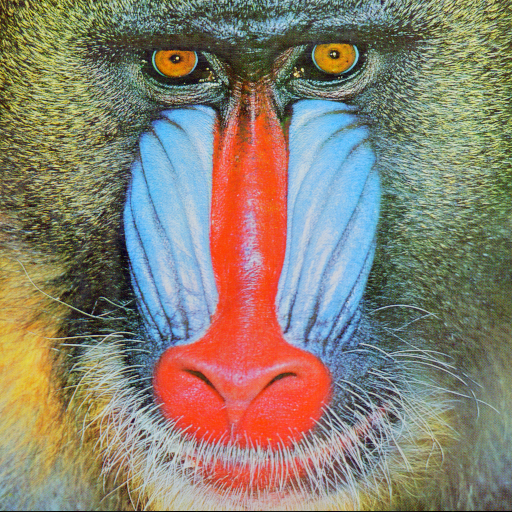
\includegraphics[width=.3\linewidth]{mandrill-large.png}\quad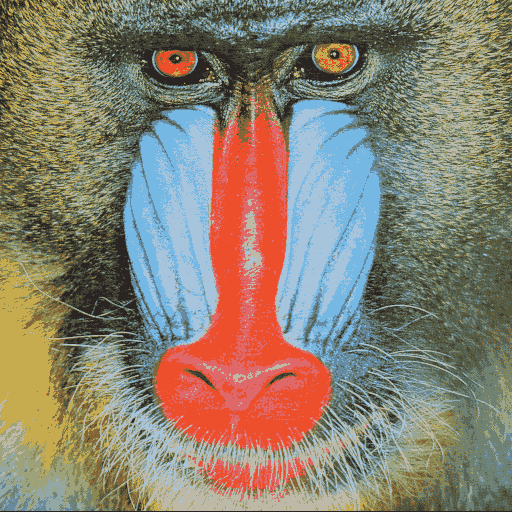
\includegraphics[width=.3\linewidth]{compressed-large-10.png}\quad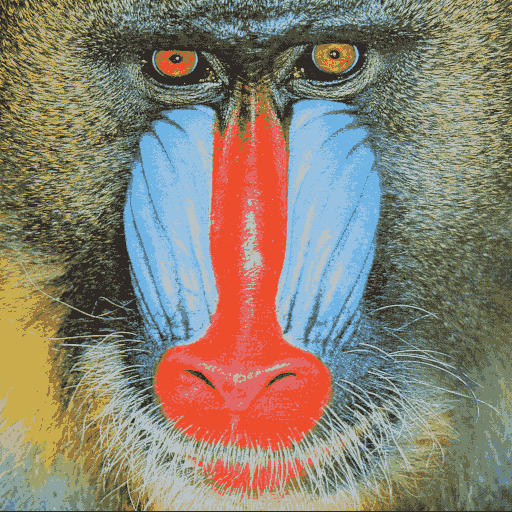
\includegraphics[width=.3\linewidth]{compressed-large.png}
\\[\baselineskip]% adds vertical line spacing
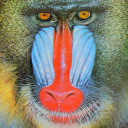
\includegraphics[width=.3\linewidth]{mandrill-small.png}\quad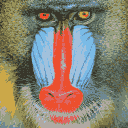
\includegraphics[width=.3\linewidth]{compressed-small-10.png}\quad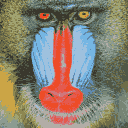
\includegraphics[width=.3\linewidth]{compressed-small.png}
\\ From left to right, they are original image, image after 10 iterations, and the converged image. The upper row is the mandrill-large. The lower row is mandrill-small.
\end{center}
In theory, file size should be smaller in the times of 6, since originally one pixel needs 24 bit but now only requires 4 bit for the encoding from the 16 colors.
\end{homeworkProblem}
%---------------------------------------------------------------------------------------
\end{document}
